%\documentclass[handout,xcolor=pdftex,dvipsnames,table]{beamer}
%\documentclass[draft]{beamer}
%\documentclass[notesonly]{beamer}
%\documentclass[notes]{beamer}
\documentclass[aspectratio=169]{beamer}\usepackage[]{graphicx}\usepackage[]{color}
%% maxwidth is the original width if it is less than linewidth
%% otherwise use linewidth (to make sure the graphics do not exceed the margin)
\makeatletter
\def\maxwidth{ %
  \ifdim\Gin@nat@width>\linewidth
    \linewidth
  \else
    \Gin@nat@width
  \fi
}
\makeatother

\definecolor{fgcolor}{rgb}{0.345, 0.345, 0.345}
\newcommand{\hlnum}[1]{\textcolor[rgb]{0.686,0.059,0.569}{#1}}%
\newcommand{\hlstr}[1]{\textcolor[rgb]{0.192,0.494,0.8}{#1}}%
\newcommand{\hlcom}[1]{\textcolor[rgb]{0.678,0.584,0.686}{\textit{#1}}}%
\newcommand{\hlopt}[1]{\textcolor[rgb]{0,0,0}{#1}}%
\newcommand{\hlstd}[1]{\textcolor[rgb]{0.345,0.345,0.345}{#1}}%
\newcommand{\hlkwa}[1]{\textcolor[rgb]{0.161,0.373,0.58}{\textbf{#1}}}%
\newcommand{\hlkwb}[1]{\textcolor[rgb]{0.69,0.353,0.396}{#1}}%
\newcommand{\hlkwc}[1]{\textcolor[rgb]{0.333,0.667,0.333}{#1}}%
\newcommand{\hlkwd}[1]{\textcolor[rgb]{0.737,0.353,0.396}{\textbf{#1}}}%

\usepackage{framed}
\makeatletter
\newenvironment{kframe}{%
 \def\at@end@of@kframe{}%
 \ifinner\ifhmode%
  \def\at@end@of@kframe{\end{minipage}}%
  \begin{minipage}{\columnwidth}%
 \fi\fi%
 \def\FrameCommand##1{\hskip\@totalleftmargin \hskip-\fboxsep
 \colorbox{shadecolor}{##1}\hskip-\fboxsep
     % There is no \\@totalrightmargin, so:
     \hskip-\linewidth \hskip-\@totalleftmargin \hskip\columnwidth}%
 \MakeFramed {\advance\hsize-\width
   \@totalleftmargin\z@ \linewidth\hsize
   \@setminipage}}%
 {\par\unskip\endMakeFramed%
 \at@end@of@kframe}
\makeatother

\definecolor{shadecolor}{rgb}{.97, .97, .97}
\definecolor{messagecolor}{rgb}{0, 0, 0}
\definecolor{warningcolor}{rgb}{1, 0, 1}
\definecolor{errorcolor}{rgb}{1, 0, 0}
\newenvironment{knitrout}{}{} % an empty environment to be redefined in TeX

\usepackage{alltt}
\mode<presentation>
\usetheme{Singapore} %Berkeley, Palo Alto, Singapore, Warsaw
%\usecolortheme{seagull}  %Beaver, dolphin, dove, lily, orchid, seagull, seahorse

%\usefonttheme{serif}
% font themes: default, professionalfonts, serif, structurebold, structureitalicserif, structuresmallcapsserif

\usepackage{graphicx}
\usepackage{pgf}
\usepackage{array}
\usepackage{tabularx}
\usepackage{booktabs}          %% Used in risk tables
\usepackage{multirow}          %% Used in decision tables
%\usepackage{beamerarticle}
%\usepackage{enumitem}
%\usepackage{beamerthemesplit}
\usepackage[T1]{fontenc}  %to use < or > in tables

\newcolumntype{Y}{>{\centering\arraybackslash}X}
\newcommand{\specialcell}[2][c]{\begin{tabular}[#1]{@{}c@{}}#2\end{tabular}}
\newcommand{\subscr}[1]{$_{\text{#1}}$}

% pdf is displayed in full screen mode automatically
%\hypersetup{pdfpagemode=FullScreen}

%\setbeamersize{sidebar width left=0.05in}
\setbeamersize{text margin left=0.1in}
\setbeamersize{text margin right=0.1in}

\setbeamertemplate{title page}
{

\includegraphics[height=0.5in]{../../images/NOAA.eps}
\hfill

\includegraphics[height=0.5in]{../../images/DFO.eps}

\vskip0pt plus 1filll
\begin{center}
{\usebeamerfont{title}\usebeamercolor[fg]{title}\inserttitle}\\
\vskip22pt
\insertauthor
\vskip22pt
\insertdate
\end{center}
\vskip0pt plus 1filll
}

%\setbeamertemplate{footline}
%{
%\begin{beamercolorbox}[wd=.05\paperwidth,ht=0ex,dp=0ex,left]{framenumber in head/foot}%
%\insertframenumber/\inserttotalframenumber
%\end{beamercolorbox}%
%}

\newcounter{saveenumi}

\newcommand{\bc}{\begin{center}}
\newcommand{\ec}{\end{center}}
\newcommand{\bn}{\begin{enumerate}}
\newcommand{\en}{\end{enumerate}}
\newcommand{\bi}{\begin{itemize}}
\newcommand{\ei}{\end{itemize}}

%% <<echo=TRUE,  message=TRUE, results='show', warning=TRUE>>=
%% opts_chunk$set(dev='cairo_ps',fig.path='knitr-cache/', fig.dpi=96, fig.width=7.5,
%%                fig.height=4, echo=TRUE, results=TRUE, message=TRUE, warning=TRUE,
%%                results='show', cache=TRUE, cache.path='knitr-cache/')


%%%%%%%%%%%%%%%%%%%%%%%%%%%%%%%%%%%%%%%%%%%%%%%%%%%%%%%%%%%%%%%%%

\title[Hake Management]{Management outcomes of the 2016 Pacific Hake stock assessment}
\author[Hicks]{Allan C. Hicks\\JTC}
%\institute{}
\date{{\footnotesize SRG meeting -- 2016}}
\IfFileExists{upquote.sty}{\usepackage{upquote}}{}
\begin{document}

\frame[plain]{
\titlepage
}

%%%%%%%%%%%%%%%%%%%%%%%%%%%%%%%%%%%%%%%%%%%%%%%%%%%%%%%%%%%%%%
\section{Introduction}
\subsection{Background}
\frame{\frametitle{Past management: Total Allowable Catch}
\begin{columns}
  \begin{column}{0.48\textwidth}
	  \bi
	    \item March 2015
      \bi
        \item JMC set an adjusted TAC = 440,000 t 
        \item Harvest rule TAC was 804,576 t 
      \ei
      \item When default HR suggests a large catch, TAC is often set less
      \item Catches are often less than the TAC
	  \ei
  \end{column}
  \begin{column}{0.48\textwidth}
    \bc 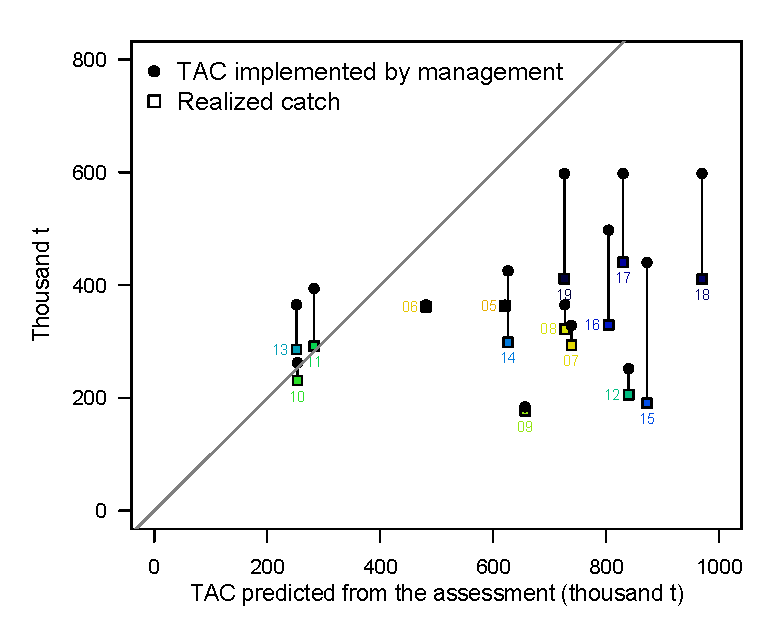
\includegraphics[width=.9\columnwidth]{Figures/ManagementResponse.eps} \ec
  \end{column}
\end{columns}
}

%---------------------------------------------------------------

\frame{\frametitle{Past management: Performance}
  \begin{columns}
    \begin{column}{0.28\textwidth}
      \bi
        \item Fishing intensity has mostly remained below target
        \item Biomass has mostly remained above target
        \item When biomass goes below target, the fishing intesity typically decreases
      \ei
    \end{column}
    \begin{column}{0.68\textwidth}
    \bc
\begin{knitrout}
\definecolor{shadecolor}{rgb}{0.969, 0.969, 0.969}\color{fgcolor}
\includegraphics[width=0.9\columnwidth]{knitr-cache/main_phase-1} 

\end{knitrout}
    \ec
    \end{column}
  \end{columns}
}

\subsection{Methods}
\frame{\frametitle{Methods}
  \bi
    \item Forecasts are for 2016, 2017, and 2018
    \bi
      \item Average fishery selectivity from 2011--2015 used in forecasts
      \item Mean weight-at-age used
      \item Used for default catch limit calculations
    \ei
    \item Equilibrium calculations
    \bi
      \item Base selectivity (used for years before 1991 as well)
      \item Mean weight-at-age
      \item Used for $B_0$, $F_{spr}$, $MSY$, etc. 
    \ei
    \item Catch streams presented for some specific cases
    \bi \item We welcome input for additional catch streams \ei
  \ei
}



%%%%%%%%%%%%%%%%%%%%%%%%%%%%%%%%%%%%%%%%%%%%%%%%%%%%%%%%%%%%%%%%%%%%
\section{Forecasts}
\subsection{Two year forecasts}
\frame{\frametitle{Harvest rule predicted catch for 2016}
\begin{columns}
  \begin{column}{0.38\textwidth}
    \bi
      \item Using the defined $F_{SPR=40\%}$ harvest rate $F_{SPR=40\%}$ harvest reate with a 40:10 adjustment the median forecasted 2016 TAC is  
      \smallskip
      \bc {\bf 804,399 t} \ec
      \smallskip
      \item 2.5\% and 97.5\% quantiles:\\ 282,653 and 1,852,960 t
    \ei
  \end{column}
  \begin{column}{0.59\textwidth}
\begin{knitrout}
\definecolor{shadecolor}{rgb}{0.969, 0.969, 0.969}\color{fgcolor}
\includegraphics[width=.95\columnwidth]{knitr-cache/main_projected_catch_density_2016-1} 

\end{knitrout}
  \end{column}
\end{columns}
}


\frame{\frametitle{Harvest rule predicted catch for 2017}
\begin{columns}
  \begin{column}{0.38\textwidth}
    \bi
      \item Using the defined $F_{SPR=40\%}$ harvest rate with a 40:10 adjustment for 2017\\
            conditioned on a fixed 2016 catch of 804,399 t, \\
            the median forecasted 2017 TAC is
      \smallskip
      \bc {\bf 889,918 t} \ec
      \smallskip
      \item 2.5\% and 97.5\% quantiles:\\ 158,071 and 3,190,424 t
    \ei
  \end{column}
  \begin{column}{0.59\textwidth}
\begin{knitrout}
\definecolor{shadecolor}{rgb}{0.969, 0.969, 0.969}\color{fgcolor}
\includegraphics[width=.95\columnwidth]{knitr-cache/main_projected_catch_density_2017-1} 

\end{knitrout}
  \end{column}
\end{columns}
}

\frame{\frametitle{Two year forecasts}
\begin{columns}
  \begin{column}{0.38\textwidth}
    \bi
      \item 
    \ei
  \end{column}
  \begin{column}{0.59\textwidth}
\begin{knitrout}
\definecolor{shadecolor}{rgb}{0.969, 0.969, 0.969}\color{fgcolor}
\includegraphics[width=.95\columnwidth]{knitr-cache/main_forecast_depletion_comparison_plot-1} 

\end{knitrout}
  \end{column}
\end{columns}
}


%%%%%%%%%%%%%%%%%%%%%%%%%%%%%%%%%%%%%%%%%%%%%%%%%%%%%%%%%%%%%%%%%%%%
\section{Decision Tables}
\subsection{Quantiles}
\frame{\frametitle{Spawning Biomass}
\begin{columns}
  \begin{column}{0.38\textwidth}
    \bi
      \item 
    \ei
  \end{column}
  \begin{column}{0.59\textwidth}
% latex table generated in R 3.2.3 by xtable 1.8-2 package
% Thu Feb 18 23:51:53 2016
\begin{table}[h]
\centering
\label{tab:es-decisions-spr}
\begingroup\fontsize{9}{11}\selectfont
\begin{tabularx}{\textwidth}{|ccc|YYYYY|}
  \hline \multicolumn{3}{|c|}{Within model quantile} & 5\% & 25\% & 50\% & 75\% & 95\%  \\ \hline \multicolumn{3}{|c|}{Management Action} &\multicolumn{5}{c|}{\textbf{Beginning of year}}\\ \cline{1-3}  & Year & Catch (t) & \multicolumn{5}{c|}{\textbf{relative spawning biomass}} \\ \hline  b: & 2016 & 180,000 &  40\% &  58\% &  75\% &  99\% & 142\% \\ 
   & 2017 & 180,000 &  42\% &  62\% &  85\% & 120\% & 206\% \\ 
   & 2018 & 180,000 &  41\% &  64\% &  90\% & 134\% & 240\% \\ 
   \hline d: & 2016 & 440,000 &  40\% &  58\% &  75\% &  99\% & 142\% \\ 
  2015 & 2017 & 440,000 &  36\% &  57\% &  80\% & 115\% & 200\% \\ 
  TAC & 2018 & 440,000 &  30\% &  52\% &  81\% & 124\% & 230\% \\ 
   \hline e: & 2016 & 760,000 &  40\% &  58\% &  75\% &  99\% & 142\% \\ 
  FI= & 2017 & 855,000 &  30\% &  50\% &  73\% & 108\% & 194\% \\ 
  100\% & 2018 & 750,000 &  17\% &  37\% &  66\% & 109\% & 216\% \\ 
   \hline f: & 2016 & 804,399 &  40\% &  58\% &  75\% &  99\% & 142\% \\ 
  default & 2017 & 889,918 &  29\% &  49\% &  72\% & 107\% & 193\% \\ 
  HR & 2018 & 785,036 &  15\% &  35\% &  64\% & 107\% & 214\% \\ 
   \hline \end{tabularx}
\endgroup
\end{table}


  \end{column}
\end{columns}
}


\frame{\frametitle{Fishing intensity}
\begin{columns}
  \begin{column}{0.38\textwidth}
    \bi
      \item 
    \ei
  \end{column}
  \begin{column}{0.59\textwidth}
% latex table generated in R 3.2.3 by xtable 1.8-2 package
% Thu Feb 18 23:51:53 2016
\begin{table}[h]
\centering
\label{tab:es-decisions-spr}
\begingroup\fontsize{9}{11}\selectfont
\begin{tabularx}{\textwidth}{|ccc|YYYYY|}
  \hline \multicolumn{3}{|c|}{Within model quantile} & 5\% & 25\% & 50\% & 75\% & 95\%  \\ \hline \multicolumn{3}{|c|}{Management Action} &\multicolumn{5}{c|}{\textbf{Fishing}}\\ \cline{1-3}  & Year & Catch (t) & \multicolumn{5}{c|}{\textbf{Intensity}} \\ \hline  b: & 2016 & 180,000 &  24\% &  33\% &  42\% &  52\% &  72\% \\ 
   & 2017 & 180,000 &  15\% &  24\% &  34\% &  45\% &  64\% \\ 
   & 2018 & 180,000 &  13\% &  23\% &  33\% &  45\% &  65\% \\ 
   \hline d: & 2016 & 440,000 &  49\% &  64\% &  76\% &  89\% & 111\% \\ 
  2015 & 2017 & 440,000 &  34\% &  51\% &  68\% &  85\% & 109\% \\ 
  TAC & 2018 & 440,000 &  31\% &  50\% &  68\% &  89\% & 115\% \\ 
   \hline e: & 2016 & 760,000 &  70\% &  87\% & 100\% & 112\% & 130\% \\ 
  FI= & 2017 & 855,000 &  58\% &  81\% & 100\% & 117\% & 137\% \\ 
  100\% & 2018 & 750,000 &  49\% &  76\% & 100\% & 123\% & 141\% \\ 
   \hline f: & 2016 & 804,399 &  72\% &  89\% & 102\% & 114\% & 132\% \\ 
  default & 2017 & 889,918 &  59\% &  83\% & 103\% & 119\% & 138\% \\ 
  HR & 2018 & 785,036 &  51\% &  79\% & 103\% & 126\% & 141\% \\ 
   \hline \end{tabularx}
\endgroup
\end{table}


  \end{column}
\end{columns}
}


%%%%%%%%%%%%%%%%%%%%%%%%%%%%%%%%%%%%%%%%%%%%%%%%%%%%%%%%%%%%%%%%%%%%
\section{Risk Tables}
\subsection{Risk}
\frame{\frametitle{Risk table definitions}
  Probabilities of "bad" things happening at different fixed catch levels
  \bi
    \item Fixed catch in all years previous, and calculate default catch in forecast year
    \item P($B_x < B_y$): Probability that biomass in forecasted year is less than specified biomass
    \item FI > 40\% target: Probability that fishing intensity in fixed catch year is greater than the target fishing intensity
    \item P($C_{y+1} < C_y$): Probability that the calculated catch in forecast year is less than the fixed catch
  \ei
}

%--------------------------------------------------------------
%\subsection{Fixed 2016 catch}
\frame{\frametitle{Risk based on fixed 2016 catch}
% latex table generated in R 3.2.3 by xtable 1.8-2 package
% Thu Feb 18 23:51:53 2016
\begin{table}[H]
\centering
\label{default}
\begingroup\fontsize{11}{12}\selectfont
\begin{tabularx}{\textwidth}{lYYYYYY}
  \toprule 
\specialcell{Catch\\in 2016 } & \specialcell{Probability\\B\subscr{2017}<B\subscr{2016}} & \specialcell{Probability\\B\subscr{2017}<B\subscr{40\%}} & \specialcell{Probability\\B\subscr{2017}<B\subscr{25\%}} & \specialcell{Probability\\B\subscr{2017}<B\subscr{10\%}} & \specialcell{Probability\\Fishing\\intensity\\in 2016\\>40\% Target} & \specialcell{Probability\\2017 Catch\\Target\\<2016 Catch} \\ \midrule 
 a:       0 &  9\% &  2\% & 0\% & 0\% &  0\% &  0\% \\ 
  b: 180,000 & 22\% &  4\% & 1\% & 0\% &  0\% &  0\% \\ 
  c: 350,000 & 32\% &  6\% & 1\% & 0\% &  6\% &  4\% \\ 
  d: 440,000 & 38\% &  7\% & 1\% & 0\% & 12\% &  9\% \\ 
  e: 760,000 & 53\% & 13\% & 3\% & 0\% & 50\% & 40\% \\ 
  f: 804,399 & 55\% & 14\% & 3\% & 0\% & 55\% & 44\% \\ 
  g: 873,000 & 57\% & 16\% & 4\% & 1\% & 62\% & 50\% \\ 
   \bottomrule 
\end{tabularx}
\endgroup
\end{table}

}

%--------------------------------------------------------------

\frame{\frametitle{Risk based on fixed 2016 catch (plot)}
  \bc
\begin{knitrout}
\definecolor{shadecolor}{rgb}{0.969, 0.969, 0.969}\color{fgcolor}
\includegraphics[width=0.9\columnwidth]{knitr-cache/forecast_risk_comparison_plot_year_1-1} 

\end{knitrout}
  \ec
}

%--------------------------------------------------------------
\frame{\frametitle{Risk based on fixed 2016 and 2017 catch}
% latex table generated in R 3.2.3 by xtable 1.8-2 package
% Thu Feb 18 23:51:53 2016
\begin{table}[H]
\centering
\label{default}
\begingroup\fontsize{11}{12}\selectfont
\begin{tabularx}{\textwidth}{lYYYYYY}
  \toprule 
\specialcell{Catch\\in 2017 } & \specialcell{Probability\\B\subscr{2018}<B\subscr{2017}} & \specialcell{Probability\\B\subscr{2018}<B\subscr{40\%}} & \specialcell{Probability\\B\subscr{2018}<B\subscr{25\%}} & \specialcell{Probability\\B\subscr{2018}<B\subscr{10\%}} & \specialcell{Probability\\Fishing\\intensity\\in 2017\\>40\% Target} & \specialcell{Probability\\2018 Catch\\Target\\<2017 Catch} \\ \midrule 
 a:       0 & 17\% &  2\% &  0\% & 0\% &  0\% &  0\% \\ 
  b: 180,000 & 30\% &  5\% &  1\% & 0\% &  0\% &  1\% \\ 
  c: 350,000 & 44\% &  9\% &  1\% & 0\% &  4\% &  5\% \\ 
  d: 440,000 & 50\% & 12\% &  3\% & 0\% & 11\% & 12\% \\ 
  e: 855,000 & 70\% & 27\% & 12\% & 2\% & 51\% & 54\% \\ 
  f: 889,918 & 71\% & 28\% & 14\% & 2\% & 54\% & 56\% \\ 
  g: 873,000 & 70\% & 29\% & 15\% & 3\% & 54\% & 56\% \\ 
   \bottomrule 
\end{tabularx}
\endgroup
\end{table}

}

%--------------------------------------------------------------

\frame{\frametitle{Risk based on fixed 2016 and 2017 catch (plot)}
  \bc
\begin{knitrout}
\definecolor{shadecolor}{rgb}{0.969, 0.969, 0.969}\color{fgcolor}
\includegraphics[width=0.9\columnwidth]{knitr-cache/forecast_risk_comparison_plot_year_2-1} 

\end{knitrout}
  \ec
}


%%%%%%%%%%%%%%%%%%%%%%%%%%%%%%%%%%%%%%%%%%%%%%%%%%%%%%%%%%%%%%%%%%%%
\section{2014 Recruitment}
\subsection{}
\frame{\frametitle{Spawning biomass for different levels of 2014 recruitment}
\begin{columns}
  \begin{column}{0.38\textwidth}
    \bi
      \item 
    \ei
  \end{column}
  \begin{column}{0.59\textwidth}
  \end{column}
\end{columns}
}


\frame{\frametitle{Fishing intensity for different levels of 2014 recruitment}
\begin{columns}
  \begin{column}{0.38\textwidth}
    \bi
      \item 
    \ei
  \end{column}
  \begin{column}{0.59\textwidth}
  \end{column}
\end{columns}
}






\end{document}
